\documentclass[conference]{IEEEtran}
\IEEEoverridecommandlockouts
% The preceding line is only needed to identify funding in the first footnote. If that is unneeded, please comment it out.
\usepackage{cite}
\usepackage{amsmath,amssymb,amsfonts}
\usepackage{algorithmic}
\usepackage{graphicx}
\usepackage{textcomp}
\usepackage{xcolor}
\usepackage{tikz}
\usepackage[normalem]{ulem}
\useunder{\uline}{\ul}{}
\usepackage{float}

\def\BibTeX{{\rm B\kern-.05em{\sc i\kern-.025em b}\kern-.08em
    T\kern-.1667em\lower.7ex\hbox{E}\kern-.125emX}}
\begin{document}

\title{CENG 435 Term Project Part 1}

\author{
\IEEEauthorblockN{Ege Özbek}
\IEEEauthorblockA{
\textit{ege.ozbek@metu.edu.tr}\\
2237709}
\and
\IEEEauthorblockN{Osman Emre Bilici}
\IEEEauthorblockA{
\textit{emre.bilici@metu.edu.tr}\\
2171353}
}

\maketitle


\section{Introduction}

As for the first part of our CENG435-Term Project , we have been assigned to employ discovery of network topology, links associated with each edge (which represents the delay between two nodes) and calculating effects of network emulation delay on end-to-end delay between two selected nodes in the network , a source and a destination node respectively. In total , in our network we have 5 nodes and  we are instructed to use User Datagram Protocol(UDP) as a mediatory network protocol.


\section{Network Topology}

\begin{figure}[htp]
    \centering
    \includegraphics[width=4cm]{tp.png}
    \caption{Assigned Network Topology}
    \label{fig:topology}
\end{figure}

Before going into any detail on design and implementation , we have to first correctly identify the network topology we are working on. To make a fairer evaluation environment and to make grading easier , all the groups work on same network topology. This topology includes 5 nodes all of which are simulated by the same machine and allows access for writing and execution of scripts on such virtual machines by SSH(Secure Shell) connection. \\
\\
Creation of network testing environment is done on Portal GENI website. Each group has to reserve a splice from a list of given computing resources. These splices are reserved for 7 days and allow creation of virtual machine nodes and links in between. All the information about topology is inscribed into RSpec files, in XML format. These files allow us easily describe and create network topologies .\\
\\
RSpec files also include link information between nodes, which are reflected as interfaces and related IP numbers in such nodes. (IP numbers assigned to each interface is of utmost importance when setting up servers and choosing target IP and ports for clients). Topology we are assigned with is fairly simple and only has 8 links in between.

\subsection{Selection of Programming Language}
Our choice for working with Python, was largely influenced by large number of built-in libraries dedicated for networking, threading and socket interfacing supported by Python. Another reason we chose python was to reduce the overhead created by boilerplate code to get us working. These choices helped us easily get on track with design and implementation.

\section{Background Information}
Socket programming is a way of connecting two nodes on a network to communicate with each other. Socket can be seen as a door between two nodes that connect to each other. \\
\\
There are two socket types for transport services: User Datagram Protocol(UDP) and Transmission Control Protocol (TCP). UDP is a protocol that does not require handshaking before the sending data,therefore there is no way for sender to verify the connection beforehand. This feature of UDP allows it to be more lightweight and faster than TCP, but it also creates an hazard for data integrity. Sometimes transmitted data can be lost or  due to congestion. \\
\\
We have implemented simple UDP application to our assignment to acquire the Round Trip Time (RTT) values. Details will be discussed in the below sections. 
\\
\section{Link Costs Discovery}

\subsection{Design for Calculating Costs}

Before the designing of our implementation, we have decided that a client-server model between nodes would be ideal. One node would act as a client and other node as a server. Client sends messages and receive echoed messages from server. The data packets travel from one node to another and travel back the source node. The duration in which this process takes place is what we looking for ant it is called Round Trip Time(RTT). In design phase, we focused on how to make operations between as optimal as possible and left the actual calculation part for implementation phase . \\
\\
In the given network topology, there are 5 nodes and 8 links. These links which connect the pairs of nodes are given as following, ($s$, $r_1$), ($s$, $r_2$), ($s$, $r_3$), ($r_2$, $r_3$), ($r_1$, $r_2$), ($r_1$, $d$), ($r_2$, $d$), ($r_3$, $d$). At the design stage, the most important question in our minds was to decide which nodes would be  server and which nodes would be client. As the RTT values of the links can be calculated with different combinations, the choice is up to design of the programmer. For example, one can choose
$s$, $d$ as client and $r_3$, $r_1$ server, $r_2$ is also server. $r_1$ and $r3$ can be client also. In this scenario $s$ ,$d$ and $r_2$ will send messages to servers and take back , then the servers are designated as $r_1$, $r_2$ and $r_3$. Calculated RTT values are outputted on the node $s$. Client $d$ also sends messages to servers $r_1$, $r_2$, $r_3$ and take back messages to node $d$, but now there are 2 uncalculated links now. Client $r1$ sends to server $r_2$. And client $r_3$ sends to server $r_2$. In this scenario, every link can be calculated. But one of the restrictions of the assignment is unsatisfied. The costs should be saved in the nodes $r_1$, $r_2$, $r_3$. \\
\\
This restriction gives us a clue about which nodes should be servers and clients. RTT values are calculated in the clients, since the data packets from the source node travel to server and come back to client. To keep track of timings , we need to know the time when data packets leave the source node and the time when the echoed data packets come back to the source node. We have realized that if we choose the nodes $r_1$, $r_2$ and $r_3$ as clients and we can choose the nodes $s$ and $d$ as servers. This approach, ignores the links between the nodes ($r_2$, $d$) and ($r_2$, $s$). We have come up with two ways to handle this problem . First one is the converting the server nodes $s$ and $d$ to both client and server. Other way is converting the node $r_2$ to act as both a server and a client. We chose the second way, since converting one node to both client and server is much more convenient for us. \\
\\
In conclusion, our approach / design can be shown in the Figure 2. The origin of the arrows represent the client nodes and the nodes which the arrow points are server nodes . As you can see the node $r_1$, $r_2$ and $r_3$ are clients and the nodes $s$, $d$ and $r_2$ are servers. \\

\begin{figure}[H]

\begin{tikzpicture}[scale=0.15]
\tikzstyle{every node}+=[inner sep=0pt]
\draw [black] (39.9,-29.7) circle (3);
\draw (39.9,-29.7) node {$r2$};
\draw [black] (67.5,-29.7) circle (3);
\draw (67.5,-29.7) node {$r3$};
\draw [black] (11.5,-29.7) circle (3);
\draw (11.5,-29.7) node {$r1$};
\draw [black] (39.9,-9) circle (3);
\draw (39.9,-9) node {$d$};
\draw [black] (39.9,-52.5) circle (3);
\draw (39.9,-52.5) node {$s$};
\draw [black] (13.84,-31.58) -- (37.56,-50.62);
\fill [black] (37.56,-50.62) -- (37.25,-49.73) -- (36.62,-50.51);
\draw [black] (13.92,-27.93) -- (37.48,-10.77);
\fill [black] (37.48,-10.77) -- (36.53,-10.83) -- (37.12,-11.64);
\draw [black] (65.1,-27.9) -- (42.3,-10.8);
\fill [black] (42.3,-10.8) -- (42.64,-11.68) -- (43.24,-10.88);
\draw [black] (65.19,-31.61) -- (42.21,-50.59);
\fill [black] (42.21,-50.59) -- (43.15,-50.47) -- (42.51,-49.69);
\draw [black] (14.5,-29.7) -- (36.9,-29.7);
\fill [black] (36.9,-29.7) -- (36.1,-29.2) -- (36.1,-30.2);
\draw [black] (64.5,-29.7) -- (42.9,-29.7);
\fill [black] (42.9,-29.7) -- (43.7,-30.2) -- (43.7,-29.2);
\draw [black] (39.9,-26.7) -- (39.9,-12);
\fill [black] (39.9,-12) -- (39.4,-12.8) -- (40.4,-12.8);
\draw [black] (39.9,-32.7) -- (39.9,-49.5);
\fill [black] (39.9,-49.5) -- (40.4,-48.7) -- (39.4,-48.7);

\end{tikzpicture}
\caption{Design for Calculating Costs}
\end{figure}
\\

\subsection{Link Costs Implementation}
As we have mentioned in previous sections , for our implementation we decided to use Python. Due to the fact that we need to send packets and listen for them from multiple sources, we have decided to go for a multi-threaded approach. Thanks to Python's threading package creating , passing arguments and waiting for execution to complete was really easy. 

As for our scripts , we have decided to follow a common pattern for our scripts that will separately run on each node. Depending on a node's role in our discovery order, a node may run a Client script, a Server script or both of them (but to a node doesn't get to be both a server and a client to same target node. ex/ in our designed discovery order $r2$ node serves as a client to $s$ and $d$, but a server to $r1$ and $r3$). Although we are using Python , we have decided to employ a main function-like wrapper to make sure that we do not run any code by mistake. 

For our general implementation we have decided to employ an Object Oriented approach to avoid code repetition. For this reason each server and client class basically wraps a worker thread with connectivity information (for server interface IP and which port to listen to , for client target server IP and port number) provided from main portion of our code.

First step in our implementation was to identify the IP's and ports that each server will use. This information was provided to us by teaching assistants with RSpec file. From GENI website we can easily inspect the interfaces each node has and to which link it belongs. 

Our design choice required us to set up nodes $s$, $r2$ , $d$ as servers. Down below link informations of each server node is given with their respective interface index number, interface IP and port numbers.\\

$s$ $\longrightarrow$ 0 - 10.10.1.1:20000\\
  $\longrightarrow$ 3 - 10.10.2.2:20001\\
  $\longrightarrow$ 4 - 10.10.3.1:20002\\
     
$d$ $\longrightarrow$ 7 - 10.10.4.2:10000\\
  $\longrightarrow$ 9 - 10.10.5.2:10001\\
  $\longrightarrow$ 12 - 10.10.7.1:10002\\
     
$r2$ $\longrightarrow$ 15 - 10.10.8.2:15000\\
   $\longrightarrow$  10 - 10.10.6.1:15001\\

Since we are interested in Round Trip Time (RTT), we require an echoing mechanism between a client and a server. \\
\\
This mechanism starts in client code , unlike TCP sockets UDP sockets don't require establishing a connection between client and a server, therefore client code we do not need to bind to an address for connection. We simply send packets and wait for some packet to come to our socket. \\
\\
In our server code on the other hand to listen for incoming packets we bind to interface's IP. Once we bind our socket to interfaces IP,  we can start to listen for packets. Another one of Python's advantages comes to our aid , by using socket.recvfrom() method , we easily get to access both the data from incoming packet and also the senders address information. (Specific implementation details can be found in our files with necessary comments added to them)\\
\\
To prevent clients from starting up , before there are any servers listening to them , we had to come up with a creative starting sequence. First, we started our servers $s$ and $d$, then we have activated the node $r2$ since its clients only targets $s$ and $d$ and this made sure its servers are ready to receive from $r1$ and $r3$. As the final step we have activated $r1$ and $r3$ nodes. This approach gave us the opportunity to measure RTT values of each link and we easily acquired results from $r1$, $r2$ and $r3$ nodes. The cost of the links can be shown in the table [1] in seconds.

\begin{table}[!htbp]
\caption{Costs of the links between the nodes (in seconds)}
\begin{tabular}{|l|l|l|l|l|l|}
\hline
               & \textbf{$s$} & \textbf{$r_1$} & \textbf{$r_2$} & \textbf{$r_3$} & \textbf{$d$} \\ \hline
\textbf{$s$}   &              &                &                &                &              \\ \hline
\textbf{$r_1$} & 0.0611       &                &                &                &              \\ \hline
\textbf{$r_2$} & 0.0809       & 0.141          &                &                &              \\ \hline
\textbf{$r_3$} & 0.000541     &                & 0.0811         &                &              \\ \hline
\textbf{$d$}   &              & 0.0611         & 0.0810         & 0.0005439      &              \\ \hline
\end{tabular}
\end{table}

\\
After we got the link costs we have moved on to calculate the shortest path between source and destination nodes using Dijkstra's Algorithm.

\subsection{Shortest Path Calculations (Dijkstra's Algorithm)}
\begin{table}[htbp]
\caption{Shortest Path Values with Previous Nodes}
\begin{tabular}{|c|c|c|c|c|c|}
\hline 
 & $s$ & $r_1$ & $r_2$ & $r_3$ &$ d $ \tabularnewline
\hline 
\hline 
$s & 0_s & 0,0611_s & 0,0809_s & 0,000541_s & \infty $ \tabularnewline
\hline 
$r_3 &  & 0,0611_s & 0,0809_s & 0,000541_s & 0,0011_{r_3}$ \tabularnewline
\hline 
$r_1 &  & 0,0611_s & 0,0809_s &  & 0,0011_{r_3}$ \tabularnewline
\hline 
$r_2 &  &  & 0,0809_s &  & 0,0011_{r_3} $ \tabularnewline
\hline 
\end{tabular}
\end{table}

Each row shows the selecting node. Each columns show the current lowest cost from the node $s$ to the that node. Each value is indicated with letters which shows the nodes. This means that the previous node of that node can be tracked this demonstration.\\
There are two list to show visited nodes and neighbours of the current node. \\

Note that all the numbers written in these tables are given in seconds.\\
\\


Step 1:\\

The node $s$ is the starter node. After visited node $s$, our priority queue will be $[r_3,r_1,r_2]$. Because $r_3$ is the lowest possible length among $r_1$, $r_2$, $r_3$ nodes from the node $s$. Their costs are $0.0611$, $0.0809$, $0.000541$ respectively. Since the node $d$ is not reachable from the node $s$, so we have indicated the node $d$ column as $\infty$.   \\
We have visited the node $s$. \\
$visited$ = $[s]$ \\



Step 2: \\

We need to track the lowest costs as a path. Therefore, algorithm should select the node $r_3$. \\
After visited $r_3$, queue will be $[r_1,r_2]$. The neighbours of the node $r_3$ are nodes $s$, $r_2$ and $d$. The cost of reaching to the node $r_3$ from the node $s$ is known ($0.000541$). When calculating the costs of neighbour nodes, the cost of reaching to the node $r_3$ is added, so that the cost of the new nodes from the node $s$ can be calculated. \\
From the node $r_3$ to the node $r_1$ is not available, so current value will remain unchanged from the previous step. \\
From the node $r_3$ to the node $r_2$, the cost of the link between these two nodes is $0.0811$. If the cost of reaching to the node $r_3$ is added, the cost of the reaching $r_2$ by way of $r_3$ from the node $s$ will be $0.0811$ + $0.000541$ = $0.081641$ $sec$. Since it is bigger than the previous value $0.0809$ $sec$, it will be not updated. It means that reaching the node $r_2$ by way of the node $r_3$ is not profitable than the other way. \\
From the node $r_3$ to the node $d$, the cost of the link between these two nodes is $0.0005439$ $sec$. When this value added to the $0.000541$, the cost of the reaching the node $d$ from the node $s$ will be $0.0010849$ $sec$.  \\
Since, the previous value of the $d$ column is infinity which is bigger than the found value, now it can be updated as $0.0010849$ $sec$. Since it is reached from the node $r_3$, in the column, we indicated the node near the value. \\
We have visited the node $r_3$. \\
$visited$ = $[s,r_3]$ \\



Step 3: \\

Algorithm continue from the queue. Since we know the target is the node $d$, we can pass to append the node $d$ to queue. It is meaningless because there will be a loop between the node $d$ and others. So we pass the node $d$ stage. But on the iteration tables you can see. \\
According to queue, the node $r_1$ will be visited. After visited $r_1$, queue will be $[r_2]$. The neighbours of the node $r_1$ are the nodes  $s$, $r_2$, $d$. The cost of reaching to the node $r_1$ from the node $s$ is $0.0611$ $sec$. This value added to the cost of the link between neighbours of the node $r_1$ and $r_1$. \\
From the node $r_1$ to the node $r_2$, the cost from the starter node to $r_2$ is $0.0611$ + $0,141$ = $0.2021$ $sec$. This cost is bigger than the cost of the between the node $s$ and $r_2$ ($0.0809$), so it will not be updated. The column of the node $r_2$ will be same as the value from previous step. \\
From the node $r_1$ to the node $d$, the cost of the link between $r_1$ and $d$ is $0.0611$ $sec$. When this value added to the cost of reaching the node $r_1$ from the node $s$ ($0,141$), the cost of reaching the node $d$ by way of the node $r_1$ from the node $s$ is $0.1222$ $sec$. This value is not lower than the previous value on the column of the node $d$, so the previous value will become current value.  \\  
We have visited the node $r_1$. \\
$visited$ = $[s,r_3,r_1]$ \\

Step 4: \\

Last element of the queue is $[r_2]$. The node $r_2$ will be visited. The cost of the reaching the node $r_2$ is  $0.0809$ $sec$. The neighbours of the node $r_2$ are $r_3$, $r_1$ , $s$ and $d$. All of the values except the cost of between $r_2$ and the node $d$ is calculated in above. The cost of between $r_2$ and the node $d$ is $0.0810$ $sec$. If we add them up, we obtain $0.1619$ $sec$ which is bigger than the previous step for column $d$. Thus, the column $d$ value remain unchanged. \\
 $visited$ = $[s,r_3,r_1, r_2]$ \\
The queue is empty now. \\

To conclude, according to table [2], shortest path length from the node $s$ to the node $d$ is $0.0011$ $seconds$. To find shortest path we can track the table. $0,0011_{r_3}$ shows the previous node before the node $d$. Thus, $r_3$ is the previous node before the node $d$. Shortest path length for  $r_3$ is $0,000541_{s}$. Previous node before the node $r_3$ is node $s$. Therefore, $s$ - $r_3$ - $d$ is the shortest path from $s$ to $d$. 
\\

To understand the steps, you can see the iteration tables at the below.

\begin{table}[!htbp]
\caption{Iteration 1}
\begin{tabular}{|l|l|l|l|l|l}
\cline{1-5}
     $s$ & $r_1$    & $r_2$    & $r_3$    & $d$      &                       \\ \cline{1-5}
  {\ul 0}  & $\infty$ & $\infty$ & $\infty$ & $\infty$ & $visited$ = \{ $s$ \} \\ \cline{1-5}
\end{tabular}
\end{table}


\begin{table}[!htbp]
\caption{Iteration 2}
\begin{tabular}{|l|l|l|l|l|l}
\cline{1-5}
$s$ & $r_1$    & $r_2$    & $r_3$            & $d$      &                             \\ \cline{1-5}
{\ul 0}   & $\infty$ & $\infty$ & $\infty$         & $\infty$ &                             \\ \cline{1-5}
    & $0.0611$ & $0.0809$ & {\ul $0.000541$} & $0.0011$ & $visited$ = \{ $s$, $r_3$\} \\ \cline{1-5}
\end{tabular}
\end{table}


\begin{table}[!htbp]
\caption{Iteration 3}
\begin{tabular}{|l|l|l|l|l|l}
\cline{1-5}
$s$     & $r_1$    & $r_2$    & $r_3$            & $d$            &                                  \\ \cline{1-5}
{\ul 0} & $\infty$ & $\infty$ & $\infty$         & $\infty$       &                                  \\ \cline{1-5}
        & $0.0611$ & $0.0809$ & {\ul $0.000541$} & $0.0011$       &                                  \\ \cline{1-5}
        & $0.0611$ & $0.0809$ &                  & {\ul $0.0011$} & $visited$ = \{ $s$, $r_3$, $d$\} \\ \cline{1-5}
\end{tabular}
\end{table}


\begin{table}[!htbp]
\caption{Iteration 4}
\begin{tabular}{|l|l|l|l|l|l}
\cline{1-5}
$s$     & $r_1$          & $r_2$    & $r_3$            & $d$            &                                         \\ \cline{1-5}
{\ul 0} & $\infty$       & $\infty$ & $\infty$         & $\infty$       &                                         \\ \cline{1-5}
        & $0.0611$       & $0.0809$ & {\ul $0.000541$} & $0.0011$       &                                         \\ \cline{1-5}
        & $0.0611$       & $0.0809$ &                  & {\ul $0.0011$} &                                         \\ \cline{1-5}
        & {\ul $0.0611$} & $0.0809$ &                  & {\ul }         & $visited$ = \{ $s$, $r_3$, $d$, $r_1$\} \\ \cline{1-5}
\end{tabular}
\end{table}


\begin{table}[!htbp]
\caption{Iteration 5}
\begin{tabular}{|l|l|l|l|l|l}
\cline{1-5}
$s$     & $r_1$          & $r_2$          & $r_3$            & $d$            &                                                \\ \cline{1-5}
{\ul 0} & $\infty$       & $\infty$       & $\infty$         & $\infty$       &                                                \\ \cline{1-5}
        & $0.0611$       & $0.0809$       & {\ul $0.000541$} & $0.0011$       &                                                \\ \cline{1-5}
        & $0.0611$       & $0.0809$       &                  & {\ul $0.0011$} &                                                \\ \cline{1-5}
        & {\ul $0.0611$} & $0.0809$       &                  & {\ul }         &                                                \\ \cline{1-5}
        &                & {\ul $0.0809$} &                  &                & $visited$ = \{ $s$, $r_3$, $d$, $r_1$, $r_2$\} \\ \cline{1-5}
\end{tabular}
\end{table}


\section{End-to-end Delay Experiment}

\subsection{Experiment Design and Node Netem Setup}

This experiment shows us a technique for testing the performance of applications over a virtual network. We emulate the delay with NetEm (Network Emulator). These emulation delays are experienced over the shortest path that we found in the previous section. In this section, details will be discussed. \\

In our assignment, we are assigned with 3 experiment with emulation delay values of $20ms$, $40ms$ and $50ms$. To emulate these 3 delays, configuration of the nodes was necessary. First of all, the nodes $r_3$, $s$ and $d$ were configured, since our shortest path is $s$ - $r_3$ - $d$. Thanks to configuration scripts given to us for the nodes $r_1$ and $r_2$ on link-cost discovery assignment as an example , we easily understood how to use $tc$ command as required. \\

The linux command $tc$ gives us the ability to characterize the links attached to nodes. $tc$ is an acronym for $Traffic\ Control$. As we can guess from its name, $tc$ command can manipulate the delay, packet loss, duplication etc. \\
 
We can see the current settings for each network interface for the node with following command: \\

\hspace{25mm} %25mm vertical space
$tc\ qdisc\ show$  \\

For example, when we run this script on the node $r_2$, we can see 4 network interface which represents the endpoint of the each link that is connected the node $r_2$. \\

In the experiment, we asked to add delays with normal distribution. We can add the delay with this $tc$ command: \\
\\
$sudo\ tc\ qdisc\ add\ dev\ eth0\ root\ netem\ delay\ 20ms\ 5ms$  \\

For experimentation we have used this line of command extensively with many variations, for example this $tc$ command emulates $20ms$ $\mp$ $5ms$ delay for the $eth0$ interface. One of the fore-mentioned variances is the $eth0$ interface. As mentioned above, for each node there are many network interfaces. According to the shortest path we found in the previous section, we run proper $tc$ commands for each node. Since our shortest path is $s$ - $r_3$ - $d$, we have configured these nodes with proper $tc$ commands. The last $tc$ command example shows that emulated delay for the eth0 interface, but in our nodes there are different interfaces. We have changed the $tc$ command, $eth0$ was removed and new network interface took place. The new $tc$ command, that we could use for the node $r_3$, is in the below: \\
\\
sudo tc qdisc add dev \$s\_adapter root netem delay 20ms 5ms \\
sudo tc qdisc add dev \$d\_adapter root netem delay\ 20ms\ 5ms 
\\

But there was a mistake, when we run this script, there were gaps between time differences that we calculated. For instance, we sends 1000 messages, we acquired $40ms$ value for first 100 messages, but after it jumped the value $4000ms$. This gap alerted us about a mistake in our code. Later, we notice that we did not add $distribution\ normal$ to end of the $tc$ command. For each node and each experiment, we configured the nodes according to these $tc$ commands.  \\

The correct way to write this command is as following,\\
\\
sudo tc qdisc\ add dev \$d\_adapter root netem delay 20ms 5ms  normal  distribution \\

After setting up the route of $s$ $\longrightarrow$ $r3$ $\longrightarrow$ $d$ with proper emulation delays, we can continue with our routing implementation. Since only the shortest path between $s$ and $d$ nodes will be used, not all links have to be utilized.\\

\subsection{Experiment Implementation}
\\
As experiment requires us to effectively measure the time it takes for a packet to reach node $d$ from node $s$, we require a common time point to synchronize our systems clocks. For this reason before running our client and server scripts, we first make a system call using os.system() method to synchronize system clock down to millisecond precision. Parameter for system call can be found down below.\\
\\
$sudo \ ntpdate \ -u \ pool.ntp.org $\\
\\
After the synchronization process we came up with a client-repeater-server implementation. Code for our experiment implementation is fairly similar to that of discovery part, with the exception of repeater.\\
\\
As we have the client and the server synchronized we have embedded the sending time of packet into the message, and decoded it once the packet arrived to the client. This approach saved us the trouble of getting outputs of sending and receiving time data sheets and comparing them separately.\\
\\
Unfortunately as we have come to realize not all packets we send are received by our destination node. Upon further investigation , we have found out that only around 300 packets out of 1000 reaches to end node. At first we have thought that this was due to the inherent structure of the virtual network, but upon additional testing we have discovered our source node $s$ has been sending UDP packets way too fast for repeater $r_3$ to receive , resulting in data loss. \\
\\
Our solution to this problem was to employ a feedback mechanism between $s$ and $r_3$, which worked by making node $s$ wait for an acknowledgement message from node $r_3$ signalling that it's ready to receive. After this synchronization there were no other problems with our packet flow and all 1000 of our packets were accounted for. \\
\\
After getting our delay results , we have created a simple script for calculating mean , variance and 95\% confidence interval for our dataset. Code for this script can be found under the name calculator.py


\subsection{Experiment Results and Discussion}

\begin{figure}[H]
    \centering
    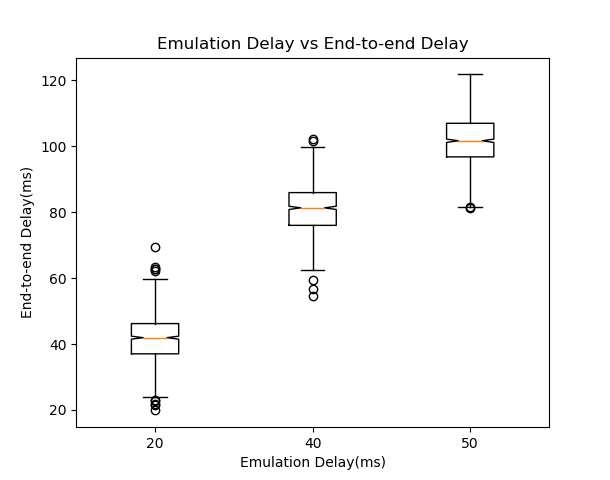
\includegraphics[width=9cm]{experiment_plot_small.png}
    \caption{Experiment Result}
    \label{fig:topology}
\end{figure}

\begin{table}[H]
\caption{Delay Means and Confidence Intervals(in ms)}
\begin{tabular}{lllll}
              & 20ms      & 40ms      & 50ms       &  \\
Mean          & 41.6867 & 80.9103 & 101.7098 &  \\
95\% interval & 2.4726  & 0.4512  & 1.3658   &  \\
              &         &         &          & 
\end{tabular}
\end{table}

Our experiment graph can be seen in their respective boxplots in the graph above, the notched parts of the boxplot represents the 95\% confidence interval. \\
\\
The result graph and related table clearly shows us that there is a linear correlation between network emulation delay and end-to-end delay.\\
\\
We believe this is due to the fact that there are two hops(link connections) in the path from source to the destination. \\
\\
We further found out that the costs associated between the nodes is fairly insignificant when compared to emulation delay. (20/40/50 ms per hop compared to 0.541 ms)



\end{document}
